%% Direttive TeXworks:
% !TeX root = ./presentazione.tex
% !TEX encoding = UTF-8 Unicode
% !TEX program = arara
% !TEX TS-program = arara
% !TeX spellcheck = it-IT

% arara: pdflatex: { synctex: yes, action: batchmode, options: "-halt-on-error -file-line-error-style" }
% arara: pdflatex: { synctex: yes, action: nonstopmode, options: "-halt-on-error -file-line-error-style" }

\documentclass[%
    % handout,      % serve per generare la versione stampabile
    % italian
]{beamer}

%% ORDINE IMPORTANTE INIZIO %%%%%%%%%%%%
\usepackage[T1]{fontenc}        % serve per impostare la codifica di output del font
\usepackage{textcomp}           % serve per fornire supporto ai Text Companion fonts
\usepackage[utf8]{inputenc}     % serve per impostare la codifica di input del font
\usepackage[
    english,        % utilizza l'inglese come lingua secondaria
    italian         % utilizza l'italiano come lingua primaria
]{babel}                        % serve per scrivere Indice, Capitolo, etc in Italiano
\usepackage{lmodern}            % carica una variante Latin Modern prodotto dal GUST
%% ORDINE IMPORTANTE FINE %%%%%%%%%%%%%%
\usepackage{xcolor}             % serve per la gestione dei colori nel testo
\usepackage{graphicx}           % serve per includere immagini e grafici
\usepackage{wrapfig}            % serve per includere figure "wrapped" nel testo
\usepackage[labelformat=empty]{caption}
\usepackage{subcaption}

\usepackage[%
    strict,             % rende tutti gli warning degli errori
    autostyle,          % imposta lo stile in base al linguaggio specificato in babel
    english=american,   % imposta lo stile per l'inglese
    italian=guillemets  % imposta lo stile per l'italiano
]{csquotes}                     % serve a impostare lo stile delle virgolette

% \usetheme{CambridgeUS}        % TODO decidi quale usare
\usetheme{Boadilla}             % serve per scegliere il layout generale dei frame
\usecolortheme{beaver}          % Per il colore va comunque bene questo
\setbeamerfont{block title}{size=\normalsize}
\setbeamerfont{block body}{size=\small}

\usepackage{pgf}
% \usepackage{pgfpages}         % serve per mettere più slide in una pagina
% \pgfpagesuselayout{4 on 1}[a4paper, border shrink=5mm, landscape]

% \usepackage[htt]{hyphenat}      % Enable hyphenation of TT text
\hyphenation{                   % Permette di sillabare bene le parole
    JavaFX
    Swing
    Micro-systems
    Script
    script
    Pack-age
    pack-age
    Manage-ment
    manage-ment
    Com-munity
    com-munity
}

\setcounter{secnumdepth}{2}     % Numera fino alla sottosezione nel corpo del testo
\setcounter{tocdepth}{3}        % Numera fino alla sotto-sottosezione nell'indice

\graphicspath{{img/}}

%% Definisco un nuovo comando per enfatizzare il testo in inglese %%%%%%%%%%%
\newcommand{\engEmph}[1] {\emph{\foreignlanguage{english}#1}}

% hyperref va caricato il più tardi possibile
\usepackage{hyperxmp}           % Simile ad hyperref
\usepackage{hyperref}           % Gestisce tutte le cose ipertestuali del pdf
\hypersetup{%
    pdfpagemode={UseOutlines},
    hidelinks,          % nasconde i collegamenti (non vengono quadrettati)
    hypertexnames=false,
    linktoc=all,        % inserisce i link nell'indice
    bookmarks=true,
    bookmarksopen,
    bookmarksopenlevel=3,
    plainpages=false,
    breaklinks,
    pdfstartview={FitH},
    pdfauthor={Niccolò Maltoni},
    pdfcopyright={Copyright (C) 2017, Niccolò Maltoni},
    pdftitle={Progettazione object-oriented di un'interfaccia grafica JavaFX per il simulatore Alchemist},
    pdfcontactcountry={Italy},
    pdfcontactemail={niccolo.maltoni@studio.unibo.it},
    pdflang={it},
    pdfsubject={Lo scopo di questa tesi è la progettazione e la successiva implementazione di un'interfaccia grafica 2D per il simulatore Alchemist. La nuova interfaccia permette di interagire con la simulazione a tempo di esecuzione e di vedere chiaramente rappresentate informazioni su di essa. In particolare, è supportata una struttura modulare di effetti che rende facilmente osservabili determinate entità del sistema ed eventuali loro proprietà: rispetto alla classe di effetti dell'interfaccia classica, la nuova tipologia di effetti non è più una funzione dal singolo nodo alla rappresentazione grafica, bensì fa riferimento all'intero ambiente, permettendo di costruire rendering complessi facilmente esportabili tramite file JSON. Si è scelto di mantenere un'interfaccia il più possibile user-friendly, mantenendo un design più simile ai simulatori a scopo videoludico per favorire l'utilizzo da parte di utenti inesperti. Lo stile estetico al quale si è deciso di allinearsi è il Material Design di Google e la libreria grafica utilizzata per l'implementazione è stata JavaFX.},
    pdfkeywords={Progettazione object-oriented, Simulazione, Java, JavaFX, Interfaccia grafica},
    pdfa
}

\title[Nuova GUI Alchemist in JavaFX]{%
    Progettazione object-oriented di un'interfaccia grafica %
    JavaFX per il simulatore Alchemist
}
\subtitle{Tesi in Programmazione ad Oggetti}
% \author[Niccolò~Maltoni]{Niccolò~Maltoni\\0000719734}
\author[Niccolò~Maltoni (0000719734)]{%
    Niccolò~Maltoni%
    \\ \small{Matricola: 0000719734}%
    \\ \vspace{10pt} \small{Realtore: Prof.~Mirko~Viroli \\Correlatore: Prof.~Danilo~Pianini}%
}
\date{12 dicembre 2017}
\institute[]{%
    Alma Mater Studiorum - Università di Bologna\\%
    Campus di Cesena%
}

%% Permette di inserire l'outline prima di ogni sezione
\AtBeginSection[]{%
    \begin{frame}<beamer>
        \frametitle{Outline}
        \tableofcontents[currentsection]
    \end{frame}
}

\begin{document}
    \begin{frame}
        \titlepage
    \end{frame}

    \section{Introduzione}\label{sec:intro}
        \subsection{Obiettivo}\label{subsec:obiettivo}
            \begin{frame}
                \frametitle{\insertsection}
                \framesubtitle{\insertsubsection}
                Lo scopo di questa tesi è la progettazione e la successiva implementazione di un'interfaccia grafica 2D più moderna e usabile per il simulatore \emph{Alchemist}.

                \medskip

                Alchemist\only<1->{\footnote{\url{http://alchemistsimulator.github.io}}} è un meta-simulatore estendibile completamente open-source che esegue su JVM, nato all’interno dell’Università di Bologna.
            \end{frame}

    \section{Analisi}\label{sec:analisi}
        \subsection{L'interfaccia classica di Alchemist}\label{subsec:oldgui}
            \begin{frame}
                \frametitle{\insertsection}
                \framesubtitle{\insertsubsection}
                \centering
                \frame{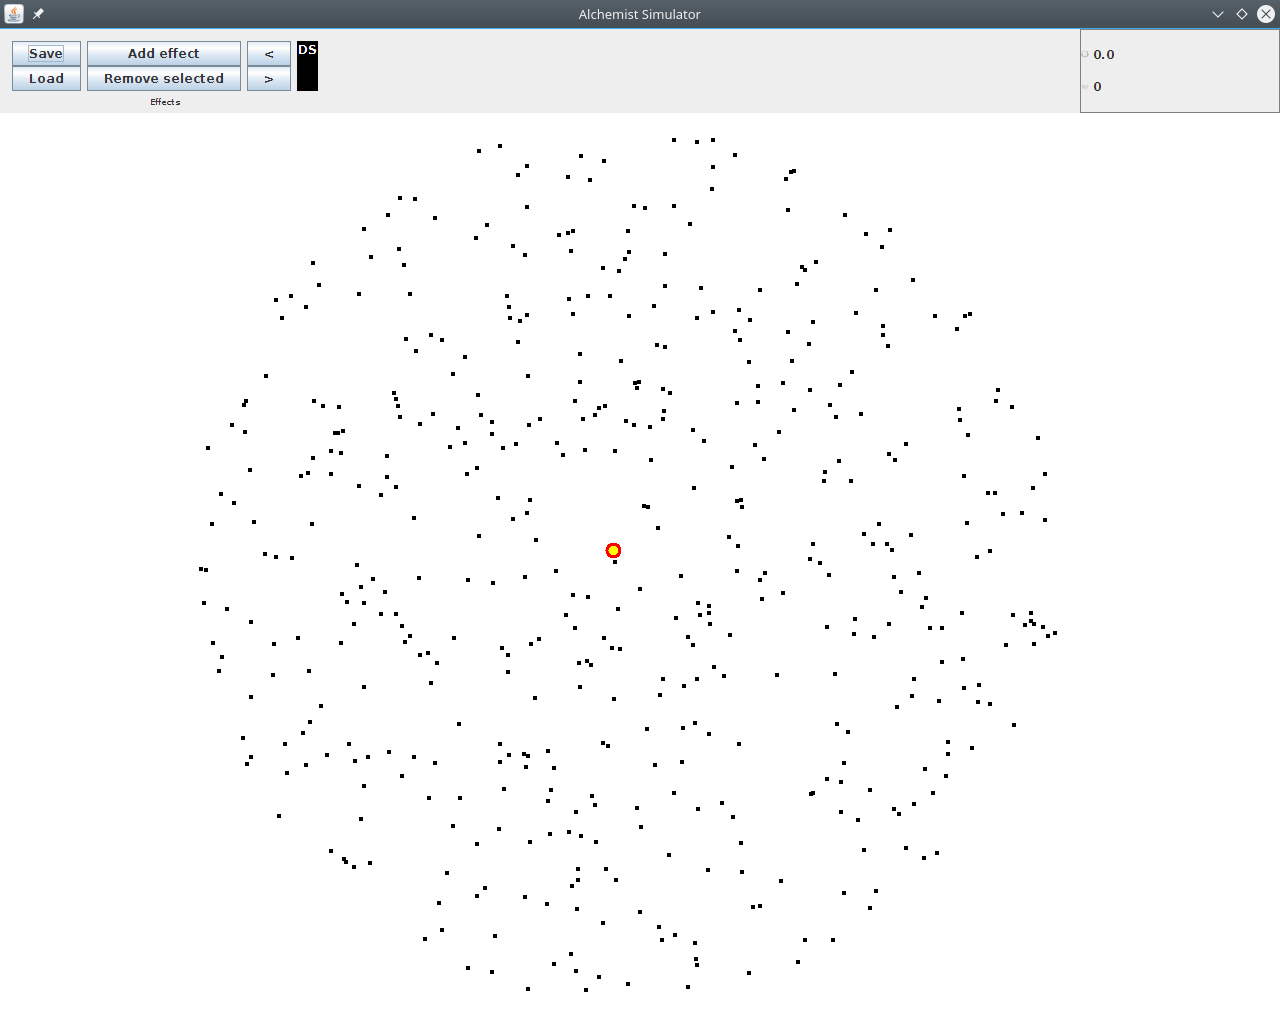
\includegraphics[scale=.27]{old/window_stopped_circle}}
            \end{frame}

            \begin{frame}
                \frametitle{\insertsection}
                \framesubtitle{\insertsubsection}
                L'interfaccia utente classica di Alchemist ha diverse criticità:

                \begin{itemize}[<+(1)->]
                    \item
                        è implementato con il framework Swing, soluzione ormai considerata \engEmph{legacy} e sostituita da JavaFX
                    \item
                        il sistema di controllo non è intuitivo
                    \item
                        l'aspetto estetico è datato e non aderisce ad alcun design grafico in particolare
                    \item
                        le capacità di rappresentazione, rappresentate dagli effetti, sono legate strettamente ai nodi e limitano la libertà di rappresentazione
                \end{itemize}
            \end{frame}

        \subsection{Requisiti \& Casi d'uso}\label{subsec:requisiti}
            \begin{frame}
                \frametitle{\insertsection}
                \framesubtitle{\insertsubsection}
                \centering
                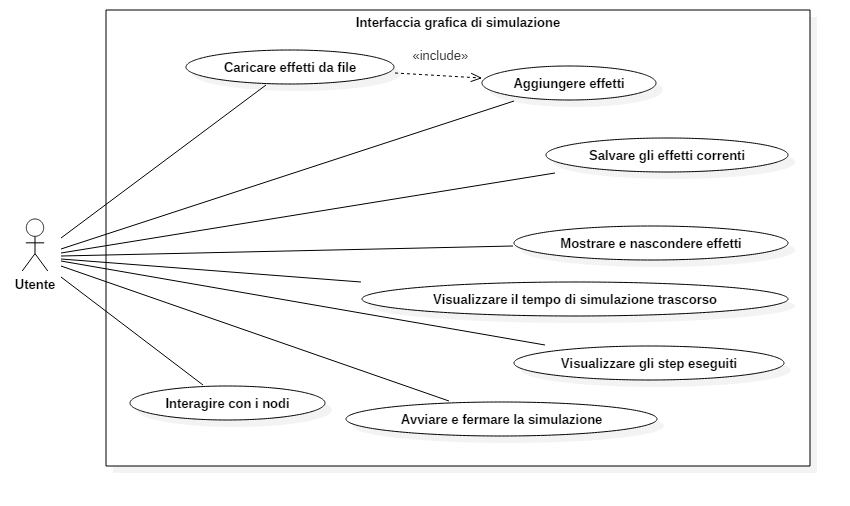
\includegraphics[scale=0.40]{uml/useCaseBeamer}
            \end{frame}

    \section{Interfaccia grafica}\label{sec:mockup}
        \subsection{Stato dell'arte e fonti d'ispirazione}\label{subsec:sota}
            \begin{frame}
                \frametitle{\insertsection}
                \framesubtitle{\insertsubsection}

                \begin{itemize}[<+->]
                    \item
                        Poiché l'obiettivo era semplificare quanto più possibile l'interazione, non sono state considerate le interfacce dei simulatori a scopo scientifico costituenti lo stato dell'arte \ldots
                    \item
                        \ldots bensì si è preferito ispirarsi a famosi simulatori videoludici, quali ad esempio Universe Sandbox
                    \item
                        Lo stile grafico è basato sul Material Design di Google
                \end{itemize}
            \end{frame}

        \subsection{Mockup}\label{subsec:mockup}
            \begin{frame}
                \frametitle{\insertsection}
                \framesubtitle{\insertsubsection}
                \centering
                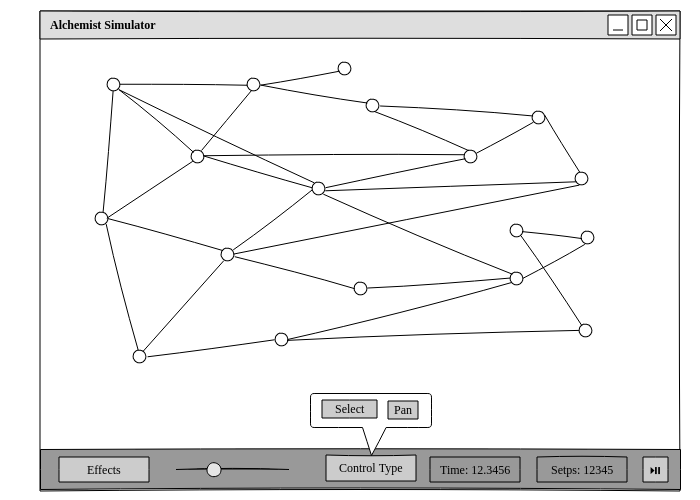
\includegraphics[scale=0.415]{mock/withNodes/window}
            \end{frame}

            \begin{frame}
                \begin{figure}[htbp]
                    \captionsetup[subfigure]{labelformat=empty}
                    \centering%
                    \begin{subfigure}{.2\textwidth}
                        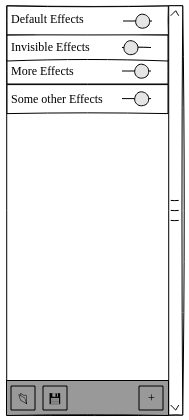
\includegraphics[scale=0.4]{mock/crop/groups}
                        \caption{Gruppi di effetti dello \engEmph{stack}}
                        \label{fig:mock:groups}
                    \end{subfigure}
                    \qquad{\LARGE$\Rightarrow$}\qquad
                    \pause
                    \begin{subfigure}{.2\textwidth}
                        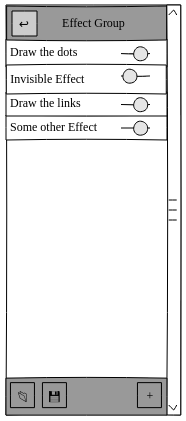
\includegraphics[scale=0.4]{mock/crop/effects}
                        \caption{Effetti di un gruppo}
                        \label{fig:mock:effects}
                    \end{subfigure}
                    \qquad{\LARGE$\Rightarrow$}\qquad
                    \pause
                    \begin{subfigure}{.2\textwidth}
                        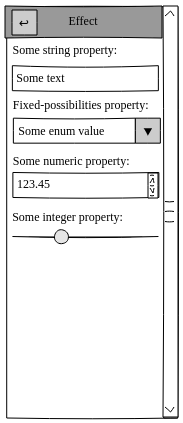
\includegraphics[scale=0.4]{mock/crop/properties}
                        \caption{Proprietà di un effetto}
                        \label{fig:mock:properties}
                    \end{subfigure}
                \end{figure}
            \end{frame}

    \section{Design e implementazione}\label{sec:newgui}
        \subsection{Caratteristiche e miglioramenti}\label{subsec:feature}
            \begin{frame}
                \frametitle{\insertsection}
                \framesubtitle{\insertsubsection}
                \centering
                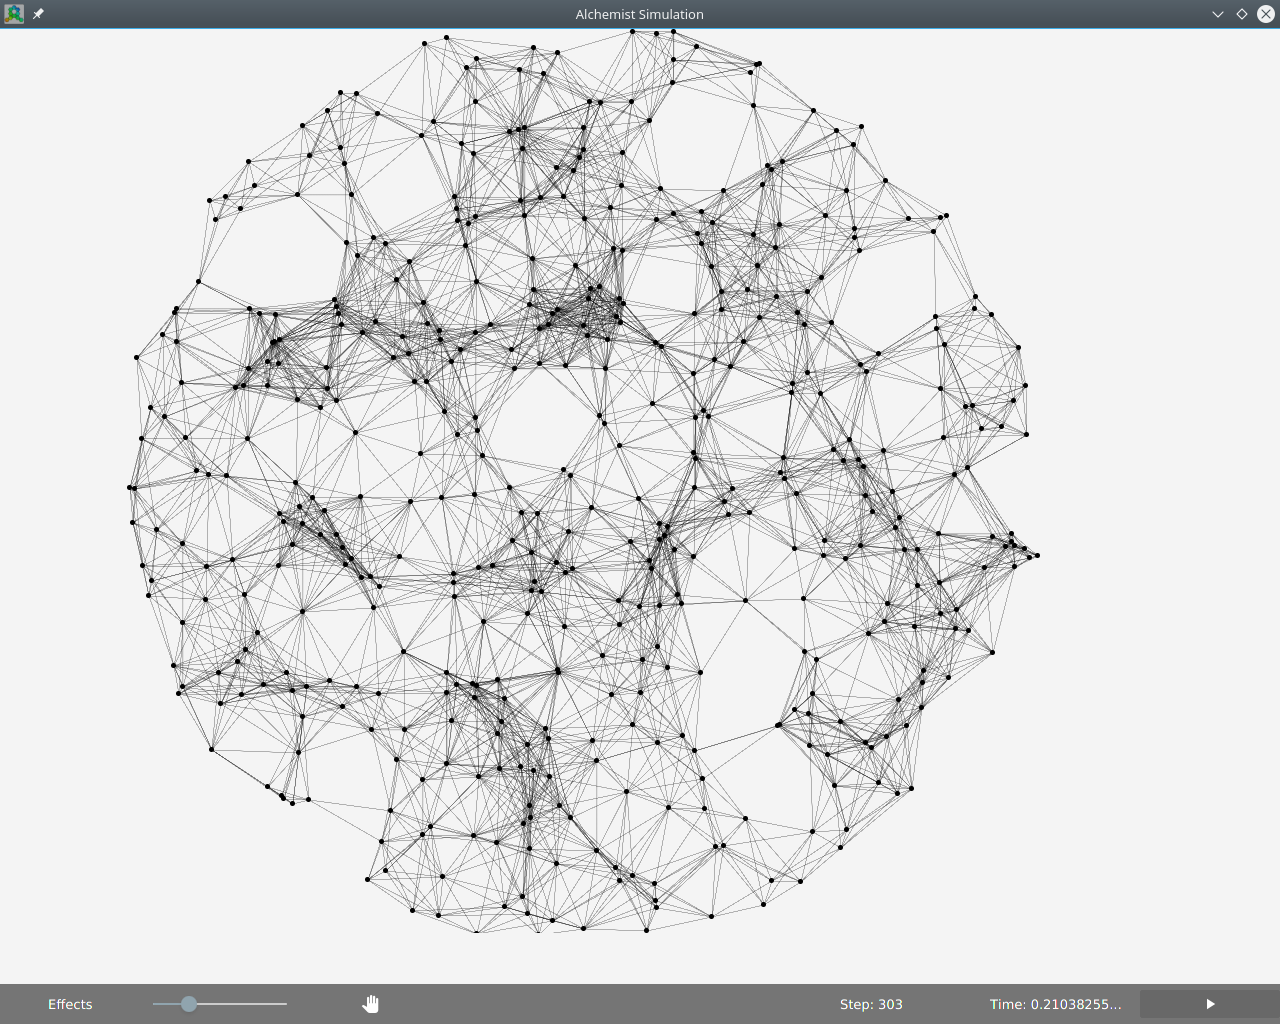
\includegraphics[scale=.27]{img/new/window_all}
            \end{frame}

            \begin{frame}
                \frametitle{\insertsection}
                \framesubtitle{\insertsubsection}
                \begin{columns}[onlytextwidth]
                    \begin{column}{.4\textwidth}
                    \begin{itemize}
                        \item<1->
                            La libreria utilizzata è JavaFX
                        \item<2->
                            è stata riprogettata l'architettura degli effetti
                        \item<3->
                            è stato introdotto l'uso di proprietà specifiche per gli effetti
                        \item<4->
                            sono stati implementati diversi monitor per la rappresentazione grafica:
                            \begin{itemize}
                              \item<5->
                                  dello stato
                              \item<6->
                                  dell'avanzamento
                              \item<7->
                                  degli effetti
                            \end{itemize}
                    \end{itemize}
                    \end{column}
                    \begin{column}{.6\textwidth}
                        \centering
                        \only<1>{%
                            \begin{block}{\centering JavaFX}
                                JavaFX è un framework che permette di costruire interfacce grafiche a partire da file FXML di layout e codice Java di controllo; rispetto a Swing:
                                \begin{itemize}
                                  \item
                                      si presta di più al pattern MVC
                                  \item
                                      scala meglio su differenti densità di pixel
                                  \item
                                      le performance sono generalmente migliori
                                \end{itemize}
                            \end{block}
                        }
                        \only<2>{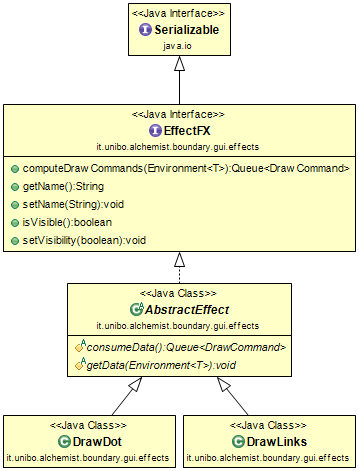
\includegraphics[scale=0.4]{uml/EffectsBeamer}}
                        \only<3>{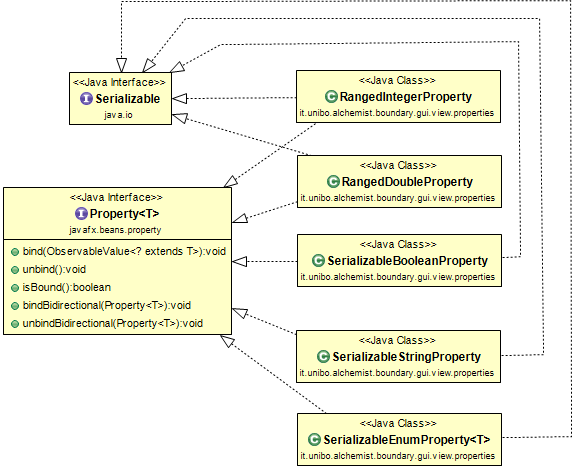
\includegraphics[scale=0.35]{uml/PropertiesSerializableBeamer}}
                        % \only<4>{}
                        \only<5>{
                            \begin{figure}[htbp]
                                \captionsetup[subfigure]{labelformat=empty}
                                \centering%
                                \begin{subfigure}{.2\textwidth}
                                    
\includegraphics[scale=0.66]{img/new/crop/PlayPause}
                                \end{subfigure}

                                \bigskip

                                \begin{subfigure}{.2\textwidth}
                                    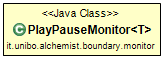
\includegraphics[scale=0.44]{uml/PlayPauseMonitor}
                                \end{subfigure}
                            \end{figure}
                        }
                        \only<6>{
                            
\includegraphics[scale=0.55]{img/new/crop/TimeStep}

                            \bigskip

                            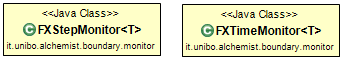
\includegraphics[scale=0.45]{uml/FXTimeStepMonitor}
                        }
                        \only<7>{
                            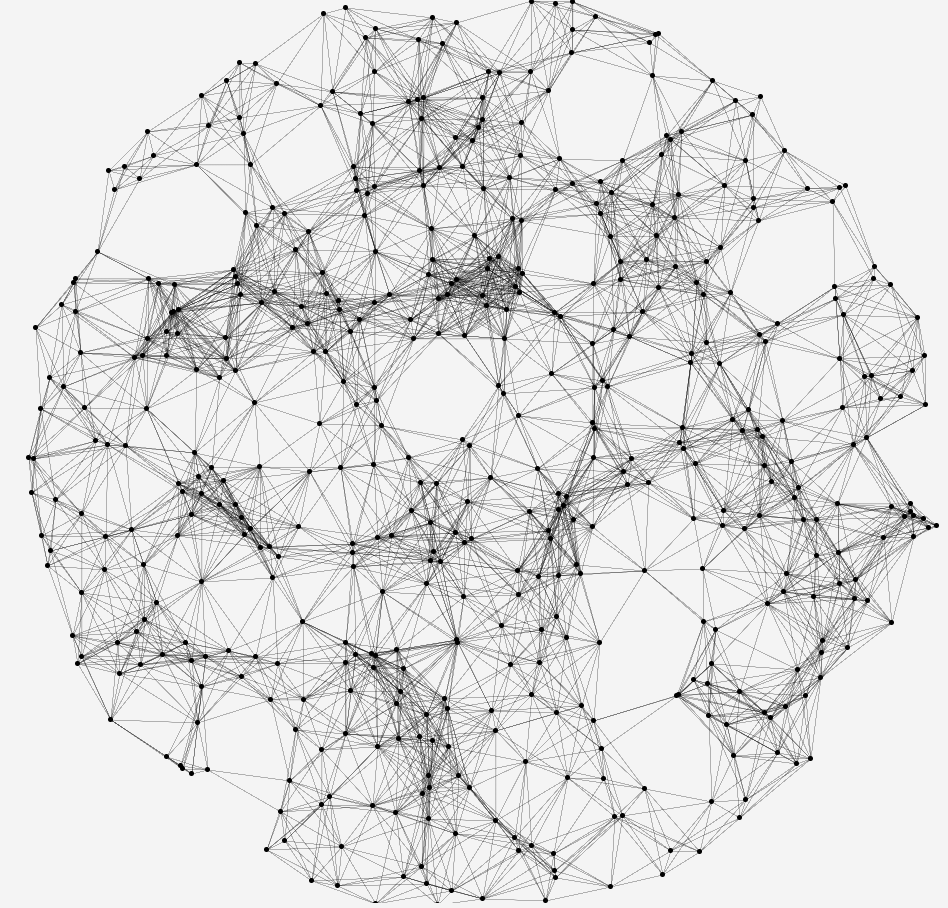
\includegraphics[scale=0.2]{img/new/crop/Canvas}

                            \bigskip

                            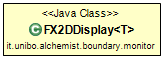
\includegraphics[scale=0.45]{uml/FX2DDisplay}
                        }
                    \end{column}
                \end{columns}
            \end{frame}

        \subsection{Coverage}\label{subsec:coverage}
            \begin{frame}
                \frametitle{\insertsection}
                \framesubtitle{\insertsubsection}
                \centering
                \frame{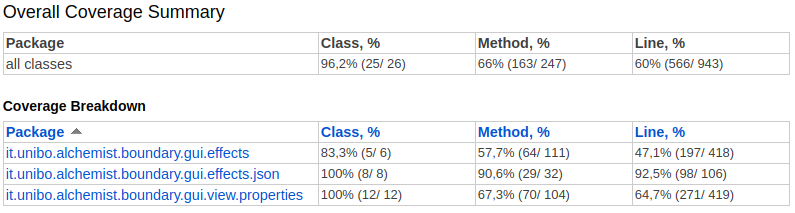
\includegraphics[scale=0.43]{fig/filtered_coverage}}
            \end{frame}

        \subsection{Prestazioni}\label{subsec:benchmark}
            \begin{frame}
                \frametitle{\insertsection}
                \framesubtitle{\insertsubsection}
                \centering
                %% Direttive TeXworks:
% !TeX root = ../presentazione.tex
% !TEX encoding = UTF-8 Unicode
% !TEX program = arara
% !TEX TS-program = arara
% !TeX spellcheck = it-IT

\begin{tabular}{ccccc}
    \multicolumn{2}{c}{\textbf{Con render}} &  & \multicolumn{2}{c}{\textbf{Senza render}} \\
     &  &  &  &  \\ \cline{1-2} \cline{4-5}
    \multicolumn{2}{|c|}{\textbf{Nuova GUI}} & \multicolumn{1}{c|}{} & \multicolumn{2}{c|}{\textbf{Nuova GUI}} \\ \cline{1-2} \cline{4-5}
    \multicolumn{1}{|c|}{Nodi + Link:} & \multicolumn{1}{c|}{$1,3153ms$} & \multicolumn{1}{c|}{} & \multicolumn{1}{c|}{Nodi + Link:} & \multicolumn{1}{c|}{1,2648ms} \\ \cline{1-2} \cline{4-5}
    \multicolumn{1}{|c|}{Solo Nodi:} & \multicolumn{1}{c|}{$0,3041ms$} & \multicolumn{1}{c|}{} & \multicolumn{1}{c|}{Solo Nodi:} & \multicolumn{1}{c|}{$0,2855ms$} \\ \cline{1-2} \cline{4-5}
     &  &  &  &  \\ \cline{1-2} \cline{4-5}
    \multicolumn{2}{|c|}{\textbf{Vecchia GUI}} & \multicolumn{1}{c|}{} & \multicolumn{2}{c|}{\textbf{Vecchia GUI}} \\ \cline{1-2} \cline{4-5}
    \multicolumn{1}{|c|}{Nodi + Link:} & \multicolumn{1}{c|}{$1,1059ms$} & \multicolumn{1}{c|}{} & \multicolumn{1}{c|}{Nodi + Link:} & \multicolumn{1}{c|}{$0,6584ms$} \\ \cline{1-2} \cline{4-5}
    \multicolumn{1}{|c|}{Solo Nodi:} & \multicolumn{1}{c|}{$0,6841ms$} & \multicolumn{1}{c|}{} & \multicolumn{1}{c|}{Solo Nodi:} & \multicolumn{1}{c|}{$0,6696ms$} \\ \cline{1-2} \cline{4-5}
\end{tabular}

            \end{frame}
    \section{Conclusioni}\label{sec:conclusioni}
        \begin{frame}
            \frametitle{\insertsection}
            \framesubtitle{\insertsubsection}
            L'obiettivo della tesi è stato per la maggior parte raggiunto: le funzionalità implementate adempiono al loro compito e l'impatto sulle performance è accettabile.

            \bigskip

            Per portare sul canale stabile il lavoro svolto è ancora necessario implementare un monitor che sia in grado di rappresentare ambienti di simulazione con mappe di sfondo e aumentare le possibilità di interazione con l'ambiente.
        \end{frame}
\end{document}
